\section{Validation of Substructure in semi-leptonic Data}
\label{sec:semilep}
Use of the top tagging algorithm described in section ~\ref{sec:toptagging} requires an understanding of how jet substructure affects kinematics in the signal region.
We use the same prescription for extracting the subjet selection efficiency and subjet energy scale as Z` $\to \ttbar$ all hadronic described in reference  \cite{7tevZprime}.

To measure the relevant substructure variables, we use single muon datasets given in table ~\ref{table:singlemusets} 

\begin{table}
\begin{center}
\bf{Single Muon Datasets}
\begin{tabular}{|p{0.7\linewidth}|p{0.3\linewidth}|}
\hline
\bf{Dataset} & \bf{Luminosity ($\pbinv$)} \\
\hline
/SingleMu/Run2012A-13Jul2012-v1/AOD & 804 \\
/SingleMu/Run2012B-13Jul2012-v1/AOD & 4429 \\
/SingleMu/Run2012C-PromptReco-v1/AOD 	 & 495 \\
/SingleMu/Run2012C-PromptReco-v2/AOD 	 & 5469 \\
/SingleMu/Run2012D-PromptReco-v1/AOD 	 & 4183 \\
\hline
Total Analyzed Luminosity &  15380 \\
\hline
\end{tabular}
\bf{Monte Carlo Datasets} \\
\begin{tabular}{|p{0.7\linewidth}|p{0.3\linewidth}|}
\hline
\bf{Dataset} & \bf{Cross section(pb)} \\
\hline
/TTJets\_MassiveBinDECAY\_TuneZ2star\_8TeV-madgraph-tauola/Summer12\_DR53X-PU\_S10\_START53\_V7A-v1/AODSIM & 225.0\\
/WJetsToLNu\_TuneZ2Star\_8TeV-madgraph-tarball/Summer12\_DR53X-PU\_S10\_START53\_V7A-v2/AODSIM & 37509.0\\
/T\_t-channel\_TuneZ2star\_8TeV-powheg-tauola/AODSIM & 56.4\\
/Tbar\_t-channel\_TuneZ2star\_8TeV-powheg-tauola/AODSIM & 30.7\\
/Tbar\_tW-channel-DR\_TuneZ2star\_8TeV-powheg-tauola/AODSIM & 11.1\\
/T\_tW-channel-DR\_TuneZ2star\_8TeV-powheg-tauola/AODSIM & 11.1\\
/T\_s-channel\_TuneZ2star\_8TeV-powheg-tauola/AODSIM & 3.79\\
/Tbar\_s-channel\_TuneZ2star\_8TeV-powheg-tauola/AODSIM & 1.76\\
/DYJetsToLL\_M-50\_TuneZ2Star\_8TeV-madgraph-tarball/Summer12\_DR53X-PU\_S10\_START53\_V7A-v1/AODSIM & 3503.71\\
\hline
\end{tabular}
\end{center}
\caption{Single Muon datasets and Monte Carlo samples used in the analysis.  These samples are used to extract variables related to jet substructure.}
\label{table:singlemusets}
\end{table}

The following selection is designed to increase the purity of $\ttbar$ events and is applied to the signal region.  We define the following cuts. 
\begin{itemize}
\item Tight Muon Selection
\begin{itemize}
\item $p_T > 45$ GeV/$c$
\item $|\eta| < 2.1$
\item The muon is from the highest Pt primary vertex
\item \verb!isTracker()! and \verb!isGlobalMuon()!
\item $\chi^2 / N_{DOF} < 10$
\item $N_{Tracker Hits} > 10$
\item $N_{Pixel Hits} > 0$
\item $N_{Muon Hits} > 0$
\item $d_0 < 0.02$ cm (with respect to the hardest DAF PV)
\item $I_{rel} < 0.12$ (using a cone size of $R=0.4$, and using $\Delta\beta$ corrections)
\item Number of matched stations $> 0$
\item no other isolated muons are allowed
\end{itemize}
\end{itemize}

The following selection is designed to simulate backgrounds in the analysis that are not simulated by 
w+jets or $\ttbar$ Monte Carlo  events and defines the sideband for the single muon analysis.  We define the following cuts.
\begin{itemize} 
\item Loose Muon Selection
\begin{itemize}
\item Can be a tracker muon OR a global muon
\item $p_T > 45$ GeV/$c$
\item Not contained in a sub-leading primary vertex
\item $I_{rel} < 0.20$
\end{itemize}
\end{itemize}

In the hemisphere opposite the isolated muon, we study the case of a dijet top, where the b and W candidate jets are both resolved.  
The following selection is required on the jets in this hemisphere for extraction of the top mass. 

\begin{itemize}
\item Hadronic Hemisphere Selection
\begin{itemize}
\item Two jets with  $p_T > 30$ $\GeVc$
\item Leading jet is required to have $p_T > 200$ $\GeVc$
\item Mass drop variable $\mu = \frac{m_1}{m_\text{jet}}$.  We require a mass drop $\mu < 0.4$, which ensures that the constituents of the merged W candidate have a roughly equal mass. 
\item Highest mass jet in the range of a W $60\GeV < M_{jet} < 130\GeV$. 
\end{itemize}
\end{itemize}
Along with these cuts, we also require one CSVM b tagged jet in the event.
The reconstructed top mass is investigated by the invariant mass of the W candidate jet and the secondary jet that is 
closest to the W candidate in $\eta/\phi$ space.  No b tagging requirement is set on the secondary jet.  The trigger selection used 
in the analysis is \texttt{HLT\_IsoMu40\_eta2p1}.  

Along with the $\ttbar$, W+jets, Z+jets, and Singletop Monte Carlo samples listed in table ~\ref{table:singlemusets}, we also model the small QCD 
contamination in the background estimate by using the loose muon id selection.  The normalization of the Monte Carlo background is then extracted from the 
cross sections listed in ~\ref{table:singlemusets}.  The QCD contribution is normalized by  
fraction fitting the $H_T$ spectrum of the leptonic hemisphere (see figure ~\ref{figs:htLep3_comp}); where $H_t \equiv E_T^{miss} + p_T^{\mu}$.  $H_t$ of the leptonic hemisphere was chosen as a fitting variable due to the assumption that this 
distribution is unrelated to substructure.  For the fit, the W+jets, Z+jets, and Singletop cross section is constrainted to between 0.8 and 1.2 of the normalization extracted 
from the cross section listed in ~\ref{table:singlemusets}.  Additionally, the b tagging scale factor and trigger efficiency scale factor is estimated to be 
0.97 and 0.93 respectively.  Because we are interested in the ratio of efficiencies, an overall normalization does not matter, and the inclusion of these 
scale factor estimations are mainly for visualization.

\begin{figure}[htcb]
\centering
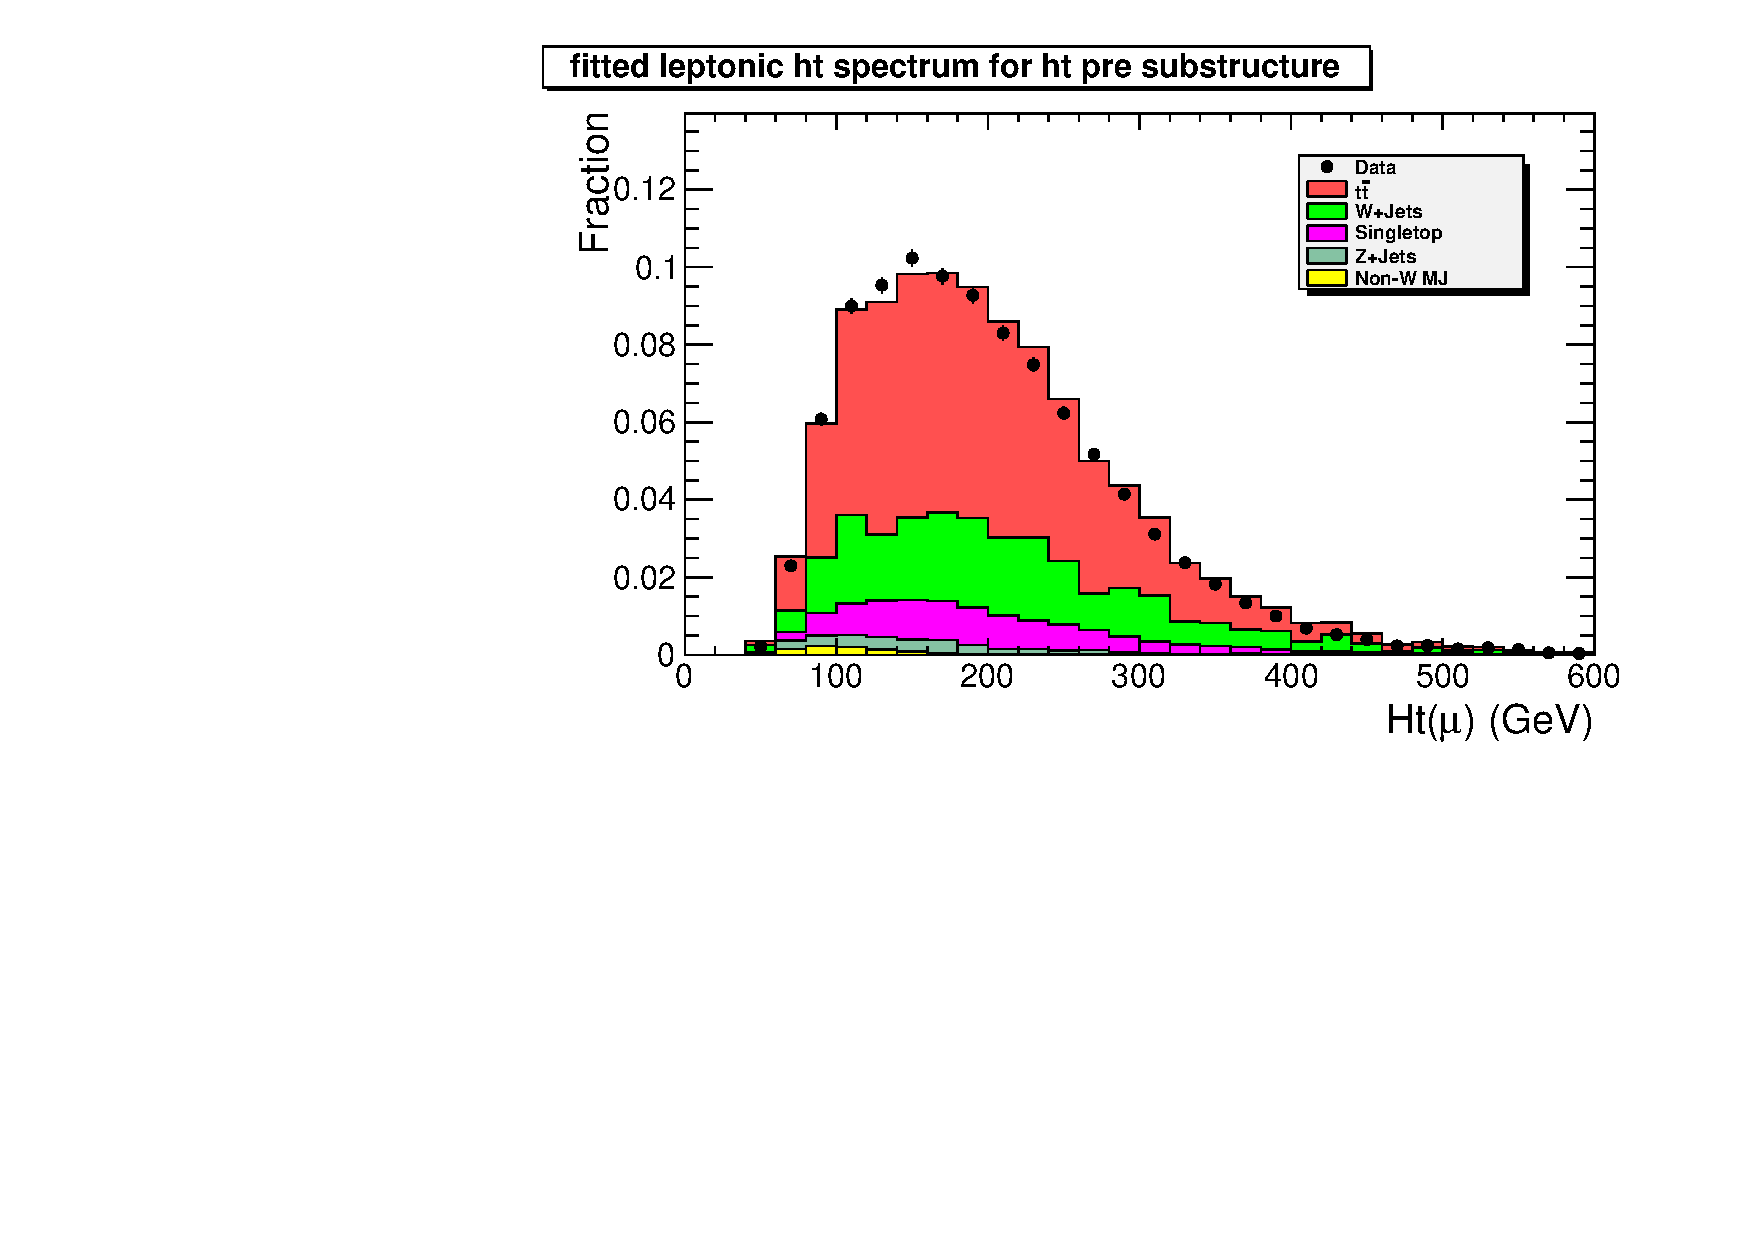
\includegraphics[width=1.0\textwidth]{figs/htLep3_comp.pdf}
\caption{Ht fit used to extract the fraction of QCD events.  This fit is performed before any substructure cuts are made.}
\label{figs:htLep3_comp}
\end{figure}


Figure ~\ref{figs:semiLepMass_mWCand} shows the highest mass jet in the hadronic hemisphere.  This jet is interpreted as originating in a W boson decay due to the
high purity of $\ttbar$ events from the previous selection.  The fits seen in figure ~\ref{figs:semiLepMass_mWCand} is a Gaussian on a very broad Guassian tail. 
The fit is performed
in both data the Monte Carlo, and from this fit we can extract the mean mass of the W boson ($M_W$).  We obtain the subjet energy scale factor by taking the 
ratio of 
$M_W$ derived from the background fit to the $M_W$ value extracted from the data fit.  From data we observe $M_W$ = 84.28$\pm$0.272 in Monte Carlo 
we observe $M_W$ = 83.662$\pm$0.164, which suggests a subjet scale factor of 1.007$\pm$0.004.

Figure ~\ref{figs:semiLepMass_muHist} shows the mass drop variable $\mu$ that is extracted from the jet pruning algorithm. From this plot we can extract the 
efficiency scale factor by measuring the ratio of efficiencies in data and Monte Carlo for a $\mu$ cut of $\mu < 0.4$.  The efficiency measured in data is 
0.498$\pm$0.003 and the efficiency measured in Monte Carlo gives 0.507$\pm$0.003, which suggests a scale factor of 0.982$\pm$0.008. From this sample, a top mass 
can be extracted by the pairwise mass of the W boson and the "closest jet" b candidate in the hadronic hemisphere described above.
The mass spectrum can be seen in figure ~\ref{figs:semiLepMass_mTopCand}.  From this, we can extract a scale factor for the W mass cut using the same procedure as 
the $\mu$ cut.
The efficiency from data is 0.550$\pm$0.004 and 0.583$\pm$0.004 from Monte Carlo.  The resulting scale factor is 0.944$\pm$0.010.  

Finally, the scale factor measurements from the $\mu$ and $M_W$ cuts are combined to give 0.927$\pm$0.013.  The type 2 scale factor is used to weight 
Monte Carlo type 2 top events in the full selection of the main analysis.

Additionally, The hadronic hemisphere can be used to extract type 1 top mass spectrum.  The cuts for this spectrum are in analogy to the main analysis.  
\begin{itemize}
\item Hadronic Hemisphere Selection
\begin{itemize}
\item Leading jet with $p_T > 400$ $\GeVc$
\item Leading jet Number of Subjets $> 2$
\item Leading jet is Minimum Pairwise mass  $> 50$ $\GeV$
\end{itemize}
\end{itemize}

The Minimum Pairwise Mass variable can be seen in figure ~\ref{figs:semiLepMass_t1MinimumPairwiseMass}, and the top mass can be seen 
in figure ~\ref{figs:semiLepMass_t1massprecut}. 
The efficiency in data for a Minimum Pairwise Mass cut of at least 50$\GeV$ is 0.607$\pm$0.017, and 0.670$\pm$0.016 for Monte Carlo giving a scale factor of 0.906$\pm$0.033.  
The efficiency for the top mass within a window of 140$\GeV$ and 250$\GeV$ in data is 0.910$\pm$0.013, and 0.890$\pm$0.013 in Monte Carlo giving a scale factor of 1.02$\pm$0.021.  
The overall scale factor for these cuts is then 0.926$\pm$ 0.039.  The type 1 scale factor is used to weight Monte Carlo type 1 top events in the full selection of the main analysis.

\begin{figure}[htcb]
\centering
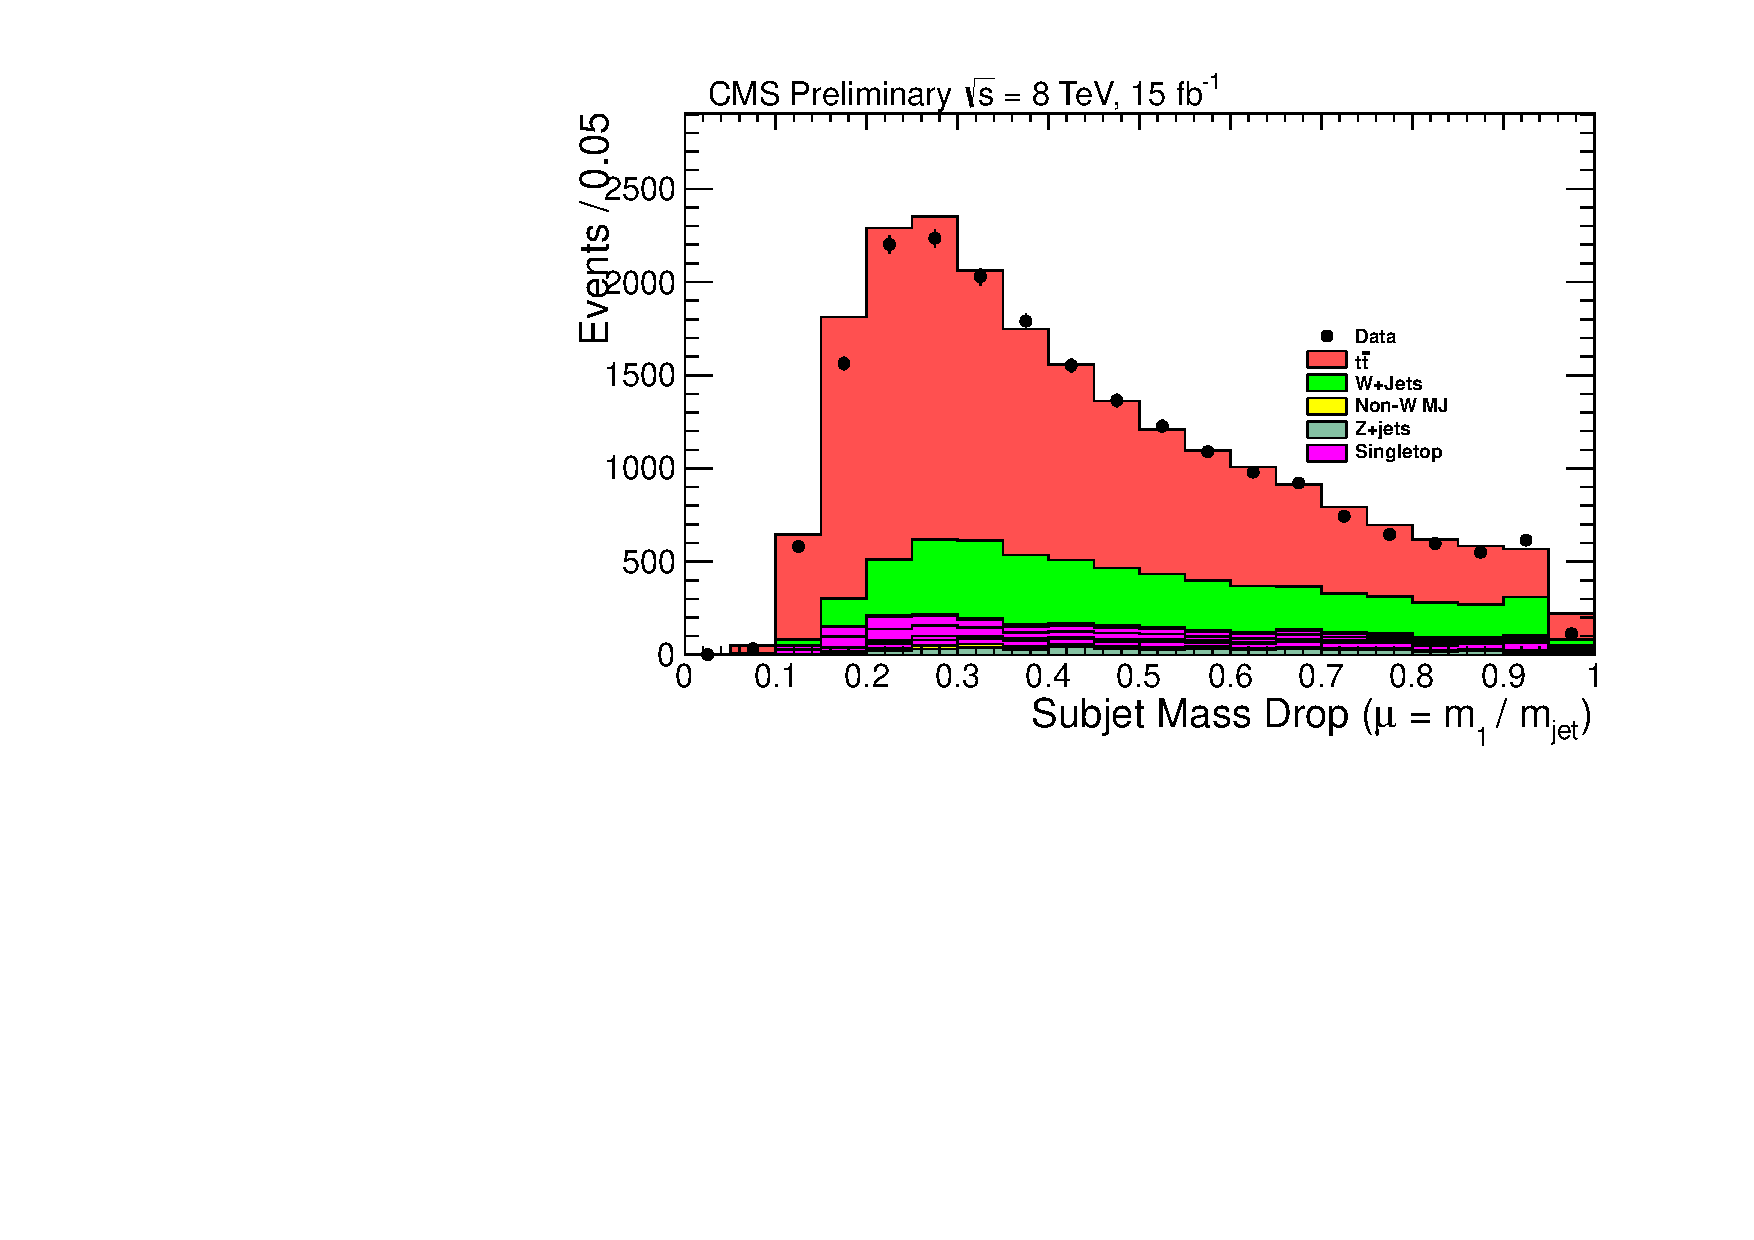
\includegraphics[width=1.0\textwidth]{figs/semiLepMass_muHist.pdf}
\caption{W candidate mass drop variable data and Monte Carlo Comparison.  The full selection for top mass requires a $\mu < 0.4$ cut.}
\label{figs:semiLepMass_muHist}
\end{figure}

\begin{figure}[htcb]
\centering
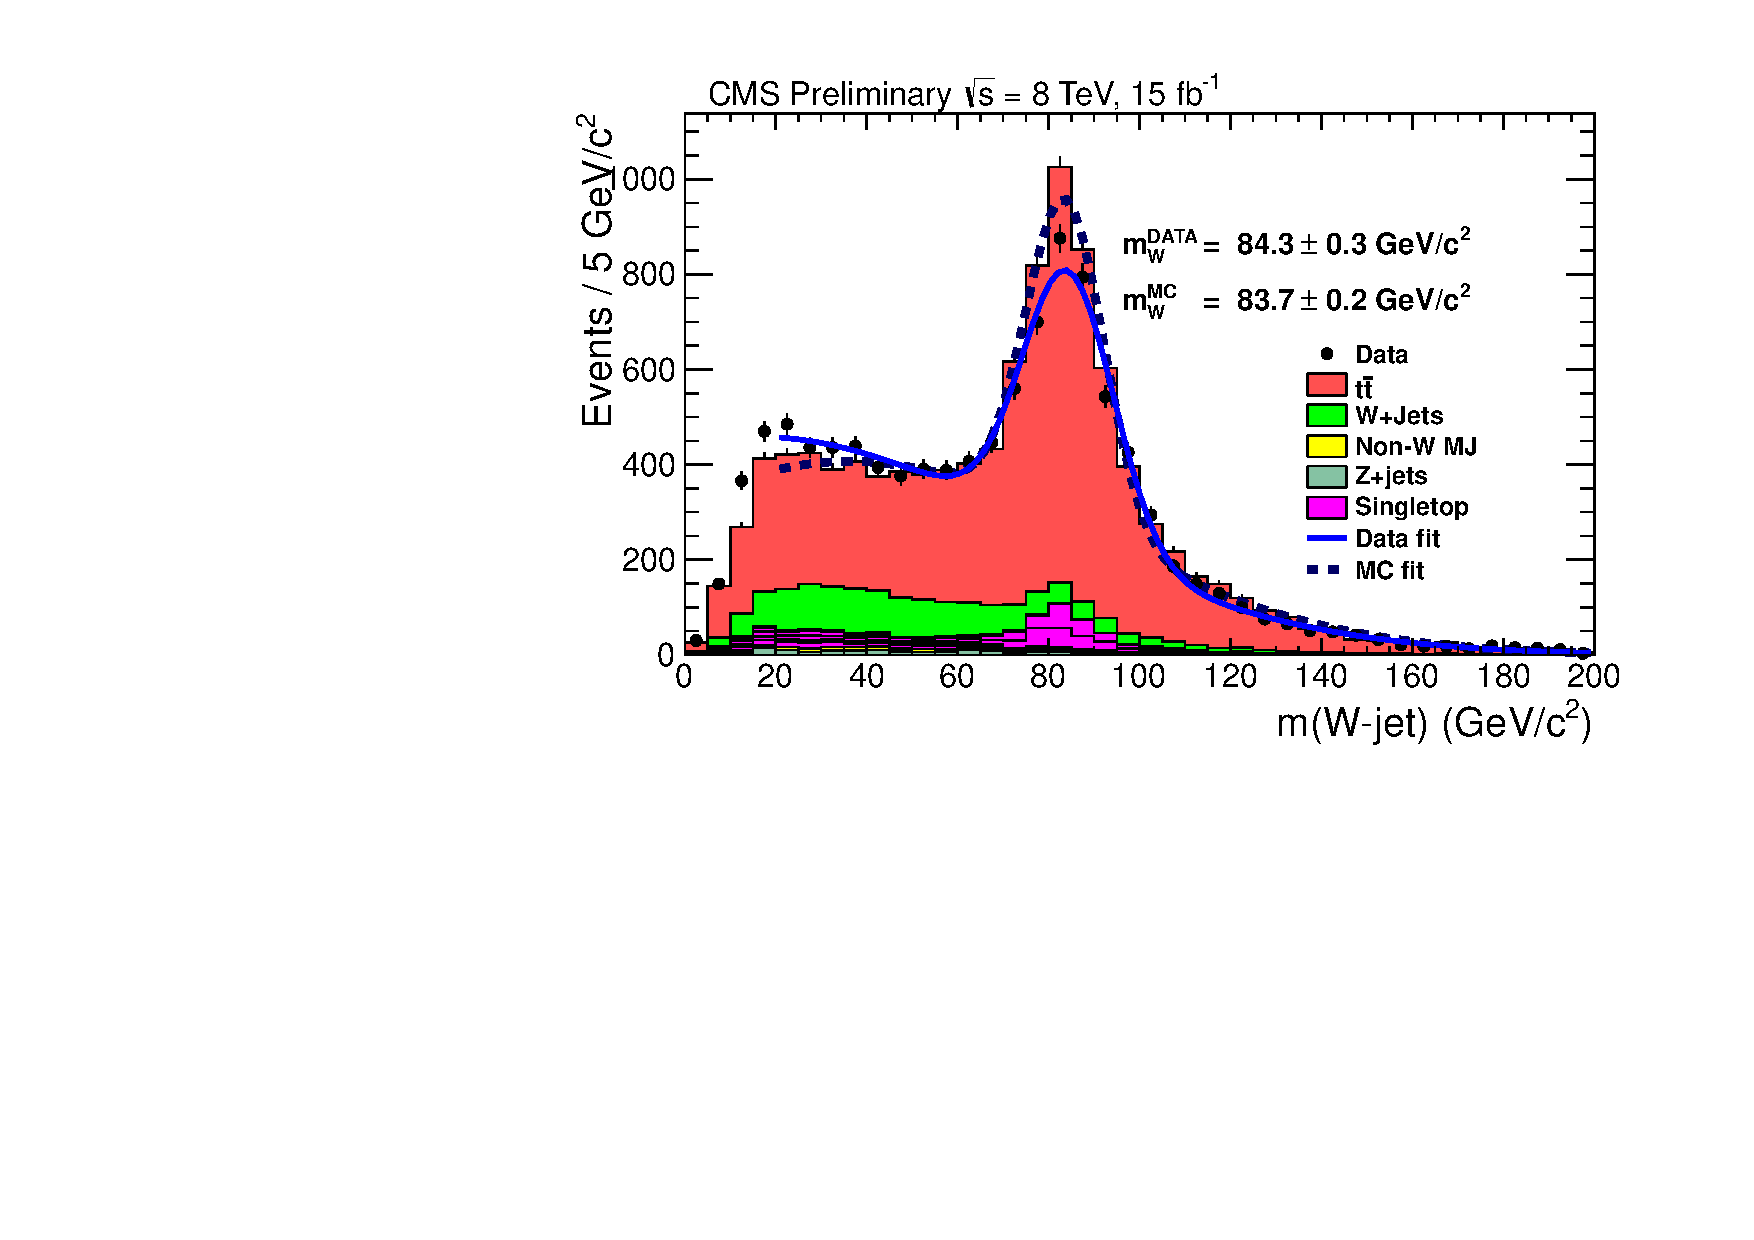
\includegraphics[width=1.0\textwidth]{figs/semiLepMass_mWCand.pdf}
\caption{W candidate mass data and Monte Carlo Comparison. The full selection for top mass requires a $60 < M_W < 130$ cut}
\label{figs:semiLepMass_mWCand}
\end{figure}

\begin{figure}[htcb]
\centering
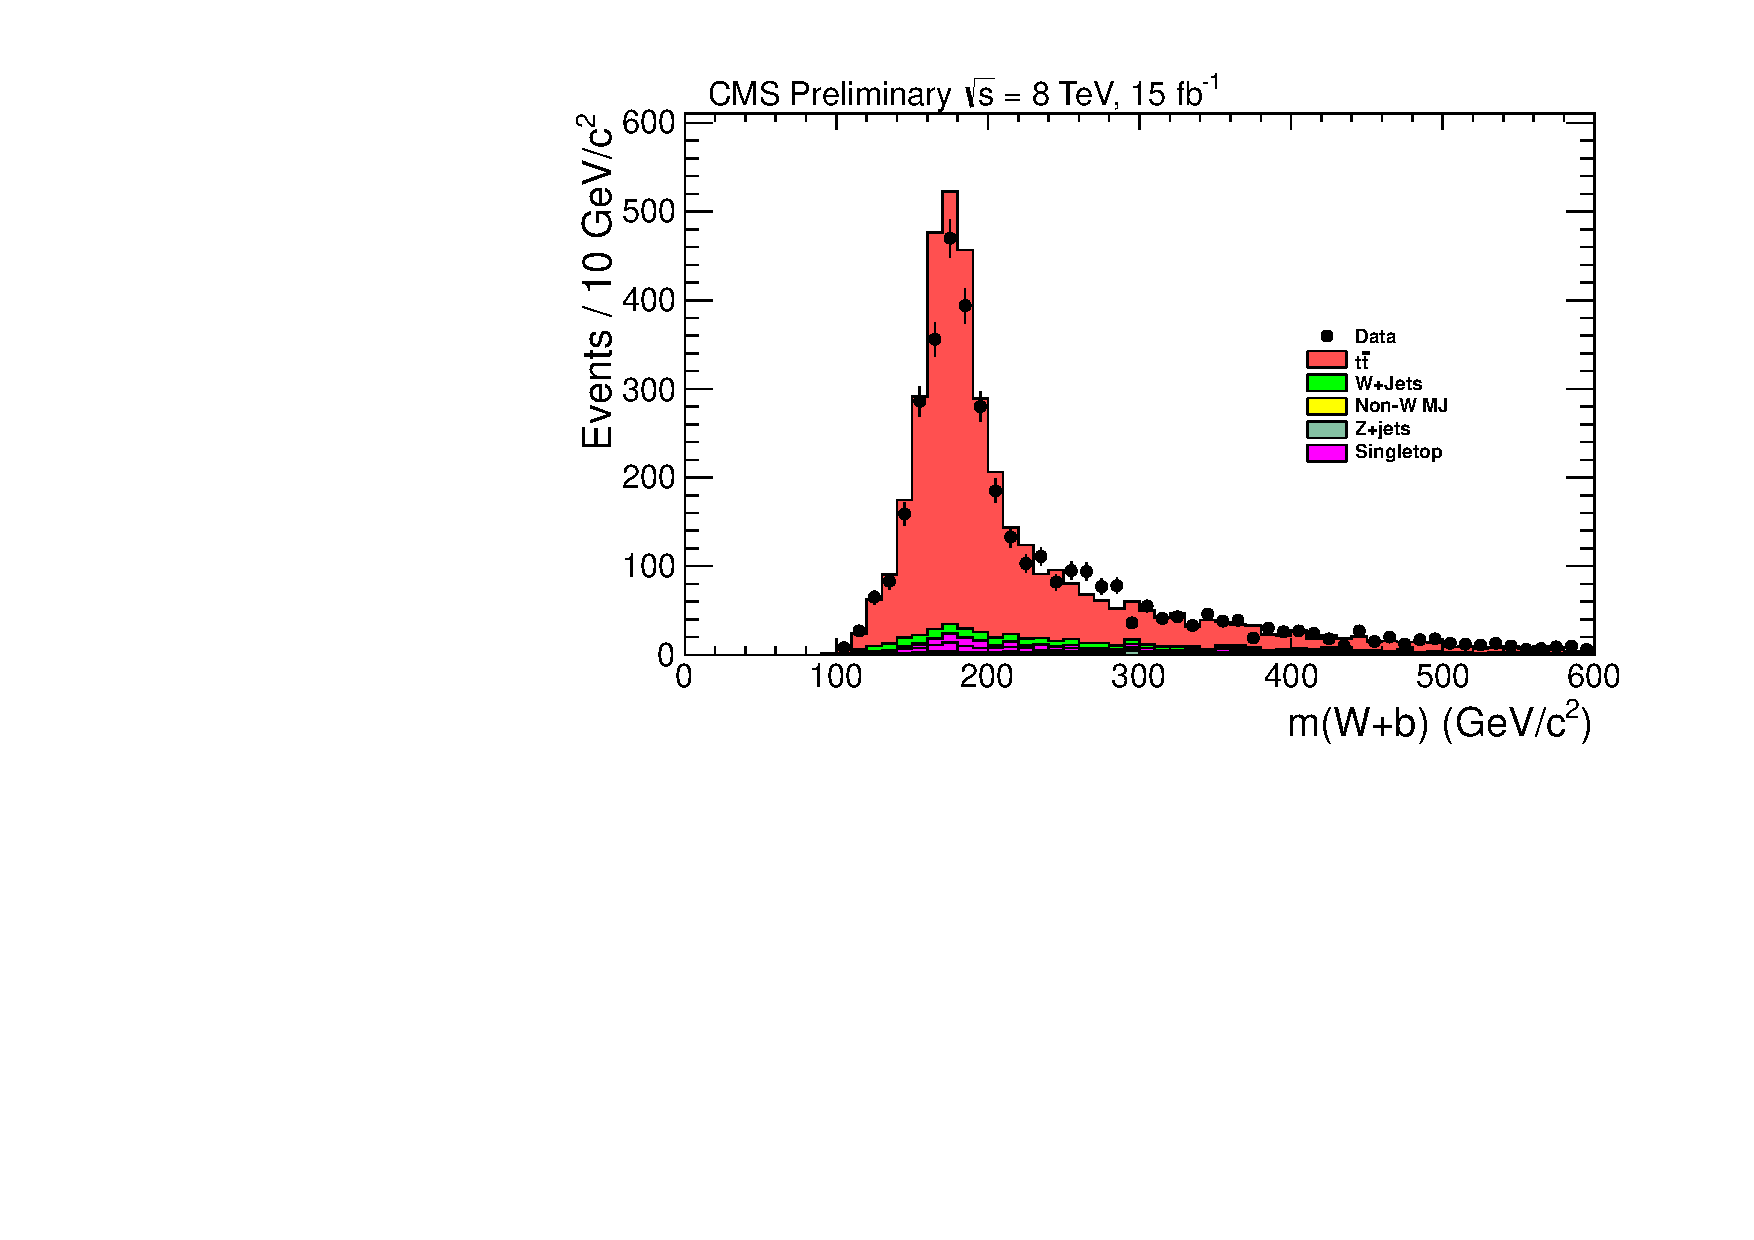
\includegraphics[width=1.0\textwidth]{figs/semiLepMass_mTopCand.pdf}
\caption{type 2 top candidate mass data and Monte Carlo Comparison}
\label{figs:semiLepMass_mTopCand}
\end{figure}

\begin{figure}[htcb]
\centering
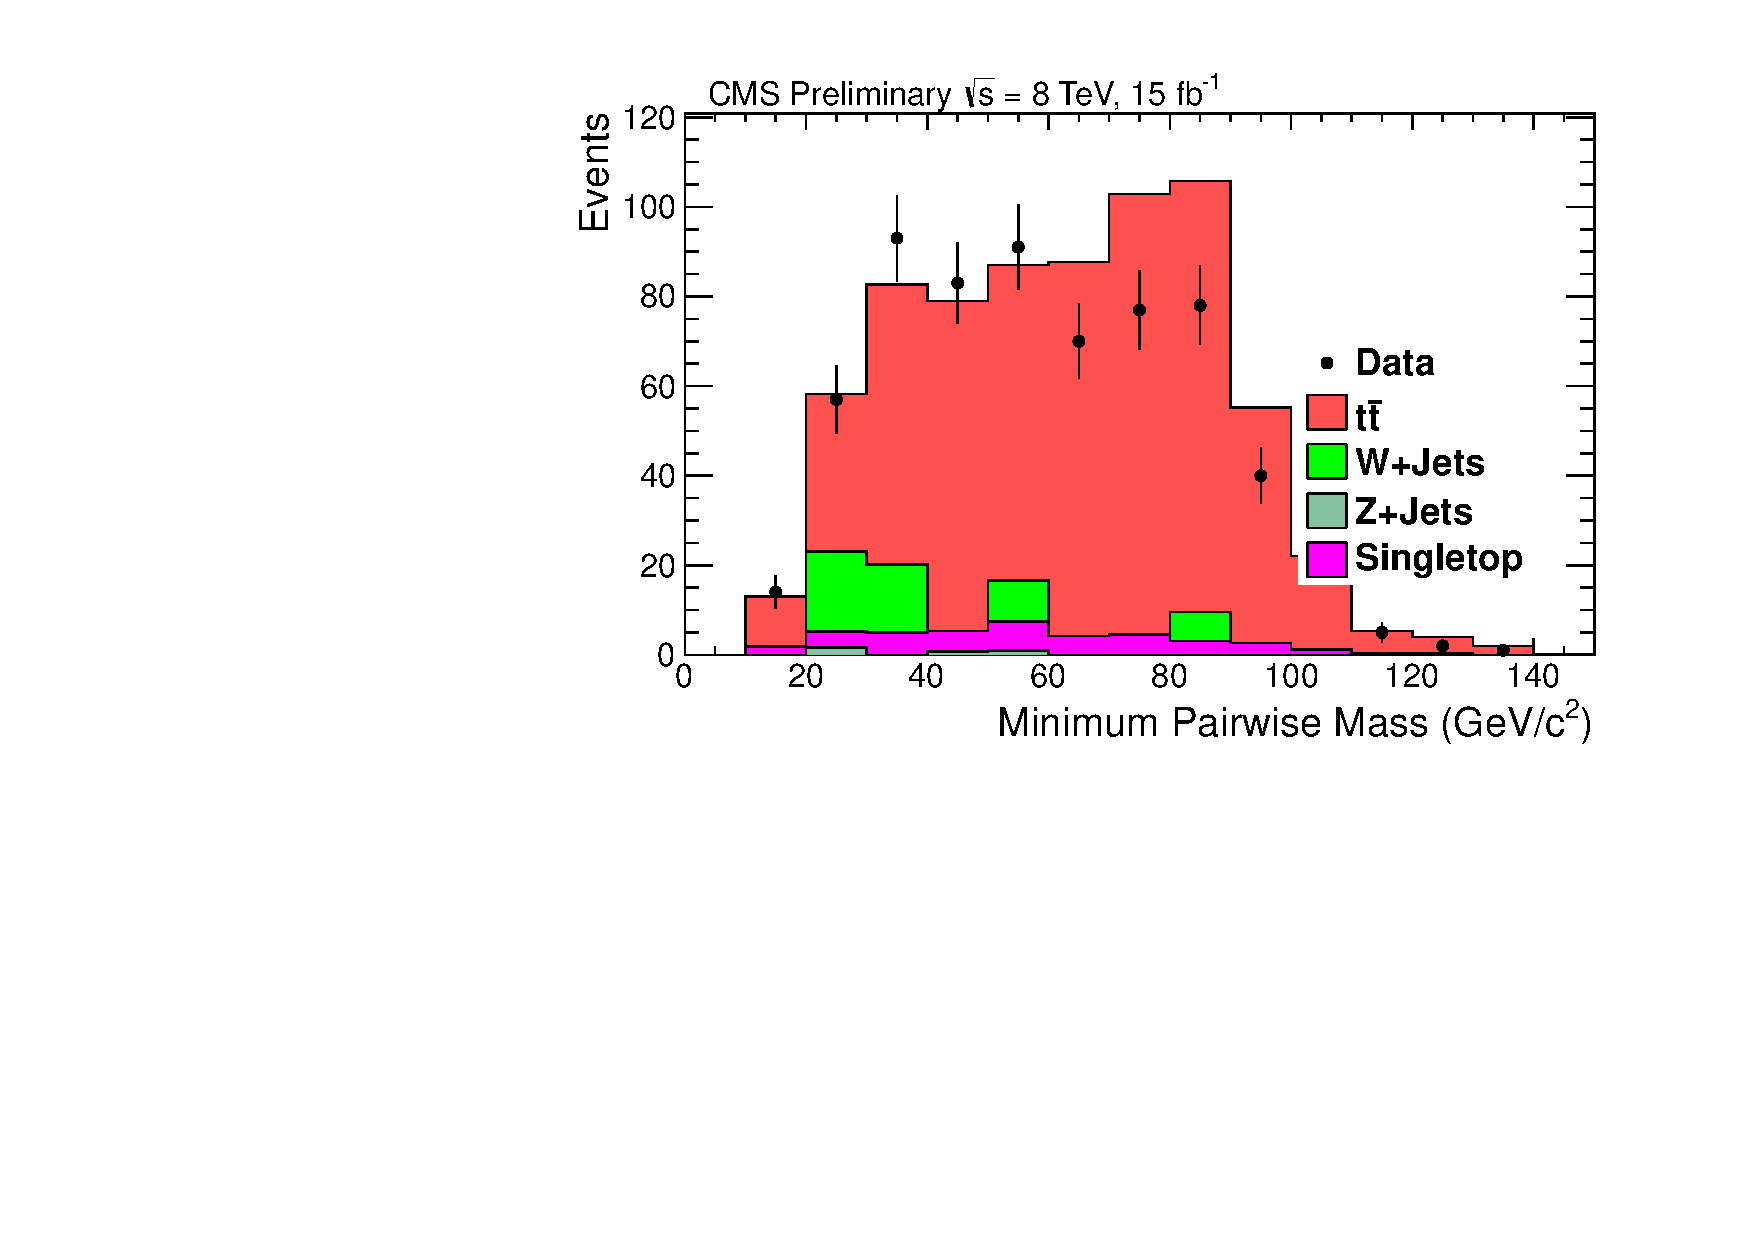
\includegraphics[width=1.0\textwidth]{figs/semiLepMass_t1MinimumPairwiseMass.pdf}
\caption{type 1 top candidate minimum pairwise mass data and Monte Carlo Comparison}
\label{figs:semiLepMass_t1MinimumPairwiseMass}
\end{figure}
\clearpage

\begin{figure}[htcb]
\centering
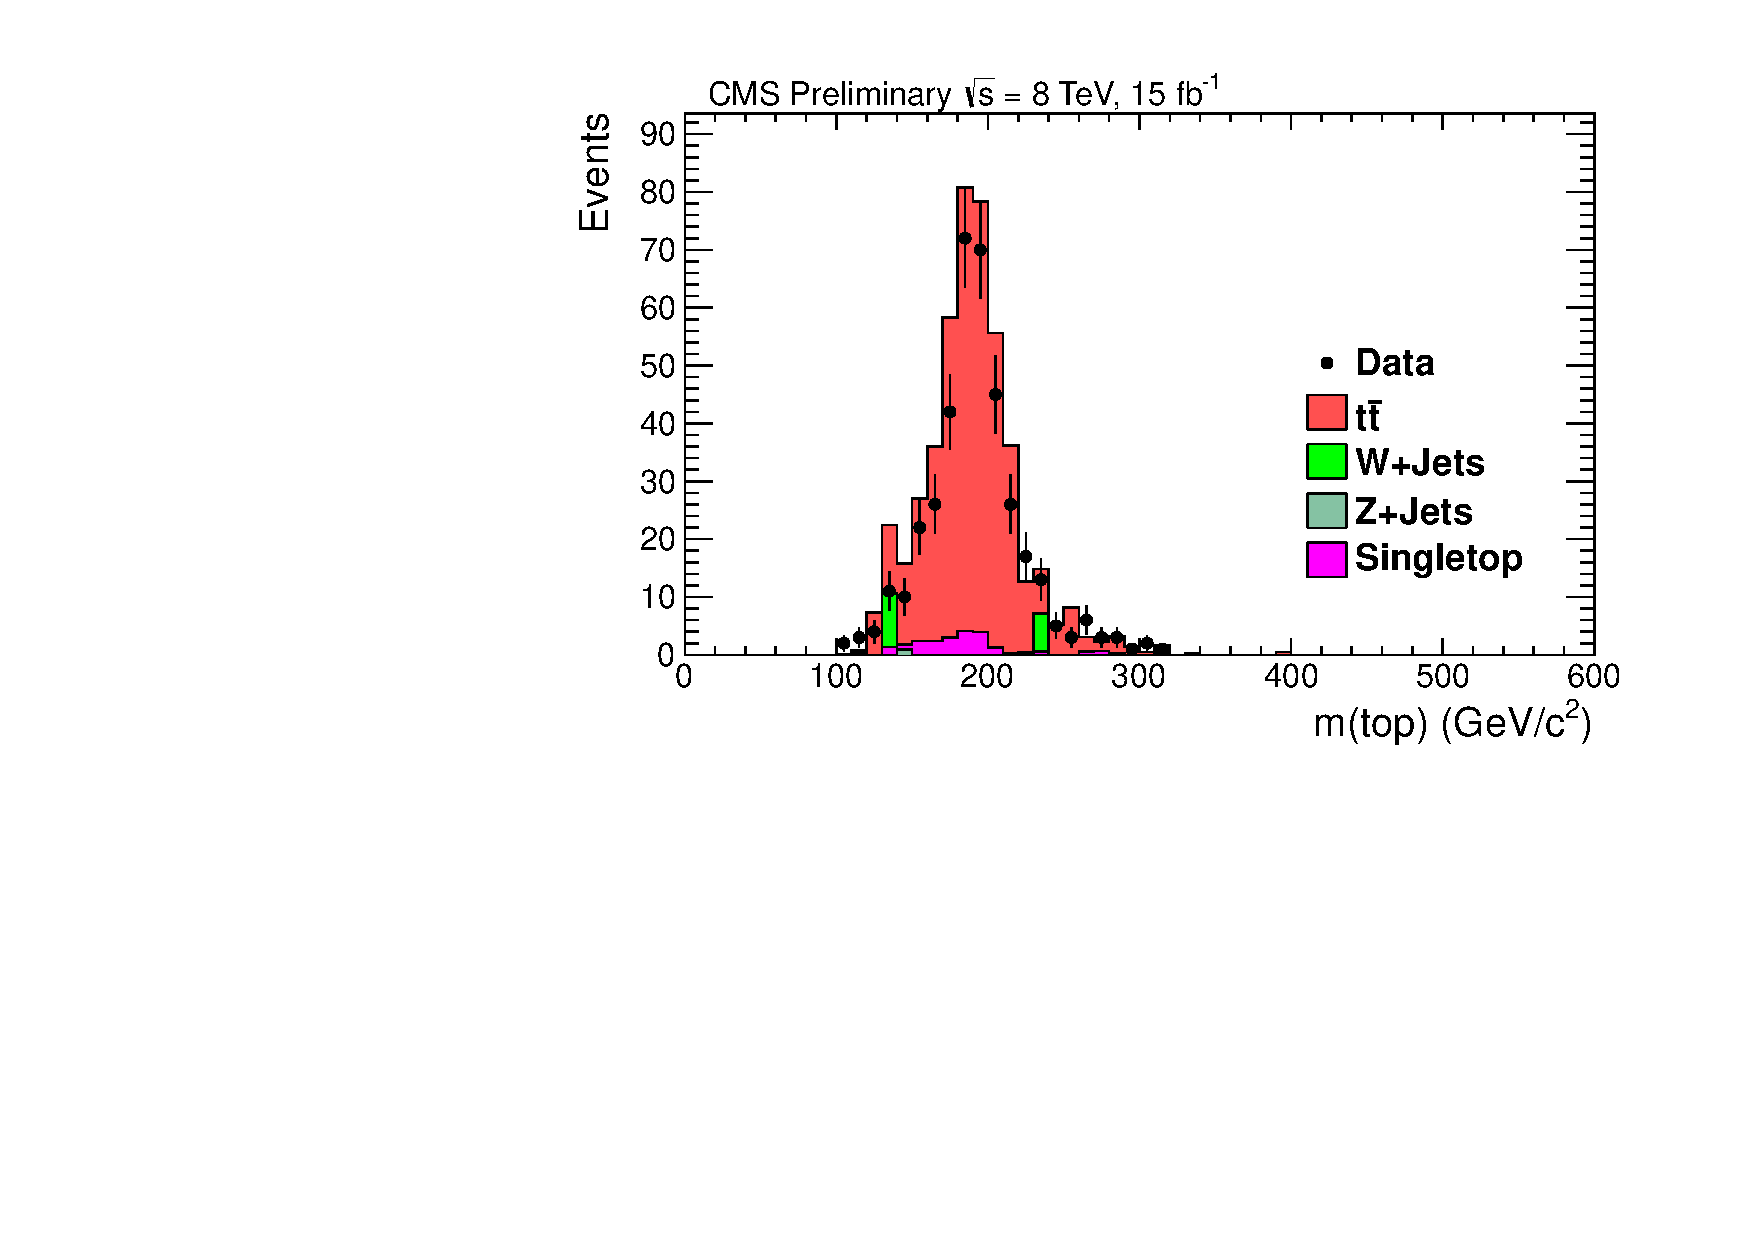
\includegraphics[width=1.0\textwidth]{figs/semiLepMass_t1TopMass.pdf}
\caption{type 1 top candidate mass data and Monte Carlo Comparison}
\label{figs:semiLepMass_t1massprecut}
\end{figure}
\clearpage
